\documentclass{article}
\usepackage{amsmath}
\usepackage{amssymb}
\usepackage{geometry}
\usepackage{titling} % Add this package for subtitle customization
\geometry{margin=1in}
\usepackage{graphicx}
\usepackage{float}

\usepackage{amsmath}
\usepackage{listings}

% Add title and subtitle for the document
\title{Exercises 01}
\pretitle{\begin{center}\Large}
\posttitle{\par\end{center}\vskip 0.5em}
\author{}
\date{}

\renewcommand{\maketitlehooka}{
  \begin{center}
    \textbf{Clustered Data Models: DATA.STAT.750}
  \end{center}
}

\begin{document}

\maketitle

\section*{Question 1}



Suppose $y_i \sim \text{Poisson}(\mu)$, where the likelihood function for independent Poisson random variables is given by:

\[
L(\mu) = \prod_{i=1}^{n} \frac{e^{-\mu} \mu^{y_i}}{y_i!}
\]

Taking  log

\[
\log L(\mu) = \sum_{i=1}^{n} \left( -\mu + y_i \log(\mu) - \log(y_i!) \right)
\]

Hypotheses:
\begin{align*}
H_0: & \ \mu = \mu_0 \\
H_1: & \ \mu = \bar{y} = \frac{1}{n} \sum_{i=1}^{n} y_i
\end{align*}

For the null hypothesis $H_0: \mu = \mu_0$, the log-likelihood is:

\[
L_0 = -n\mu_0 + \sum_{i=1}^{n} y_i \log(\mu_0) - \sum_{i=1}^{n} \log(y_i!)
\]

For the alternative hypothesis $H_1: \mu = \bar{y}$, the log-likelihood is:

\[
L_1 = -n\bar{y} + \sum_{i=1}^{n} y_i \log(\bar{y}) - \sum_{i=1}^{n} \log(y_i!)
\]


\[
-2(L_0 - L_1)
\]

Substituting

\[
-2(L_0 - L_1) = -2 \left( -n\mu_0 + n\bar{y} + \sum_{i=1}^{n} y_i (\log(\mu_0) - \log(\bar{y})) \right)
\]

Simplifying:

\[
-2(L_0 - L_1) = 2n \left( \bar{y} - \mu_0 \right) + 2 \sum_{i=1}^{n} y_i \log \left( \frac{\bar{y}}{\mu_0} \right)
\]

simplifies form:

\[
2n \bar{y} \log \left( \frac{\bar{y}}{\mu_0} \right)
\]

Thus, the likelihood ratio statistic is:

\[
-2(L_0 - L_1) = 2n \left( (\bar{y} - \mu_0) + \bar{y} \log \left( \frac{\bar{y}}{\mu_0} \right) \right)
\]






\section*{Question 3}




\begin{itemize}
    \item The log-likelihood for \textbf{Model 1} (quantitative \texttt{color}) is $-762.6794$.
    \item The log-likelihood for \textbf{Model 2} (factor \texttt{color}) is $-762.2960$.
    \item The Likelihood Ratio (LR) statistic is computed as:

    \[
    LR = 2 \times (-762.2960 + 762.6794) = 0.3834
    \]

    \item The degrees of freedom (df) difference between the two models is 2.
    \item The p-value for the LR test is $0.8256$ This means the two models are not significantly different.
\end{itemize}




In \textbf{Model 1}
\begin{itemize}
    \item The coefficient for \texttt{color} is $-0.2689$ with a p-value of $0.0282$. This means that for each unit increase in the color score, the expected log count of the number of satellites decreases by $0.2689$.
    \item This suggests a \textbf{significant negative linear relationship} between the \texttt{color} score and the number of satellites.
\end{itemize}

The p-value of approximately $0.0296$. Thus, there is no color effect.


\rule{\linewidth}{0.1mm}

\begin{itemize}

    \item The zero-inflated negative binomial model suggests that \texttt{color} does not strongly affect the zero component, and a likelihood-ratio test comparing it with the regular negative binomial model is not straightforward due to differences in the model structure.
\end{itemize}







\section*{Question 4 }


ZINB model shows that both the count of satellites and the likelihood of zero satellites are influenced by color.




\section*{Question 5 }


\begin{itemize}
    \item Fit the main-effects logistic regression model to assess the independent effects of color and weight.
     \item Fit a model including the interaction between color and weight.

     \item
Conduct a likelihood-ratio test to compare the two models and test if the interaction term significantly improves the model.

\end{itemize}


\section*{Question 6 }



\begin{figure}[H] % Ensure you use 'H' if you want it to appear exactly here
  \centering
  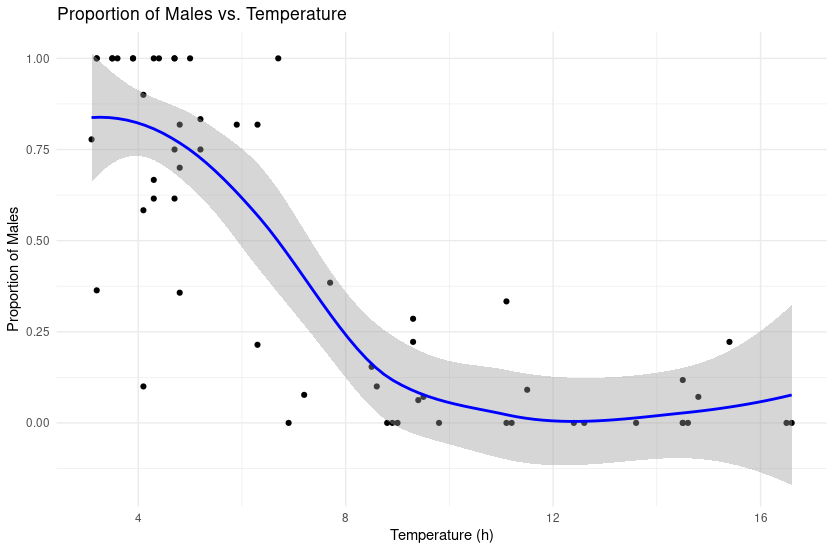
\includegraphics[width=\textwidth]{cluster_01.png}
  \caption{Plot}
  \label{fig:enter-label}
\end{figure}



a) There is a nonlinear relationship between temperature and the proportion of males.
\newline
\newline
\newline
\textbf{b}
There is a significant negative linear relationship between incubation temperature and the probability of a turtle being male.
\begin{verbatim}
Call:
glm(formula = cbind(s, n - s) ~ h, family = binomial, data = Rats)

Coefficients:
            Estimate Std. Error z value Pr(>|z|)
(Intercept)  3.66310    0.30741   11.92   <2e-16 ***
h           -0.57250    0.04733  -12.10   <2e-16 ***
---
Signif. codes:  0 ‘***’ 0.001 ‘**’ 0.01 ‘*’ 0.05 ‘.’ 0.1 ‘ ’ 1

(Dispersion parameter for binomial family taken to be 1)

    Null deviance: 509.43  on 57  degrees of freedom
Residual deviance: 205.73  on 56  degrees of freedom
AIC: 281.2
\end{verbatim}

\textbf{c)}
\begin{figure}[H] % Ensure you use 'H' if you want it to appear exactly here
  \centering
  \includegraphics[width=\textwidth]{c.png}
  \caption{Plot}
  \label{fig:enter-label}
\end{figure}


Outliers exist, with several points that go beyond the limits


\textbf{d) }


The quadratic model fits the data better than the linear model.

\begin{verbatim}
Call:
glm(formula = cbind(s, n - s) ~ h + I(h^2), family = binomial,
    data = Rats)

Coefficients:
            Estimate Std. Error z value Pr(>|z|)
(Intercept)  5.68499    0.70991   8.008 1.17e-15 ***
h           -1.17946    0.19134  -6.164 7.09e-10 ***
I(h^2)       0.03916    0.01128   3.472 0.000517 ***
---
Signif. codes:  0 ‘***’ 0.001 ‘**’ 0.01 ‘*’ 0.05 ‘.’ 0.1 ‘ ’ 1

(Dispersion parameter for binomial family taken to be 1)

    Null deviance: 509.43  on 57  degrees of freedom
Residual deviance: 195.61  on 55  degrees of freedom
AIC: 273.08

Number of Fisher Scoring iterations: 5
\end{verbatim}



\textbf{ e) }
The observed variance is significantly higher than expected, indicating potential overdispersion in the data.
\newline
\newline
\newline
\textbf{ f) }
The model provides a significantly better fit compared to the original model.
\end{document}







